\documentclass[11pt,reqno]{amsart}

\usepackage[utf8]{inputenc}
\usepackage[T1]{fontenc}
\usepackage{amsmath,amssymb,amsthm,mathtools}
\usepackage{geometry}
\geometry{a4paper, margin=1in}
\usepackage{hyperref}
\hypersetup{
    colorlinks=true,
    linkcolor=blue,
    citecolor=red,
    urlcolor=teal
}
\usepackage{tikz}
\usetikzlibrary{arrows.meta, calc}
\usepackage{microtype}
\usepackage{booktabs}
\usepackage{array}
\usepackage{tabularx}

% --- Teoremas e Estruturas ---
\newtheorem{theorem}{Theorem}[section]
\newtheorem{lemma}[theorem]{Lemma}
\newtheorem{proposition}[theorem]{Proposition}
\newtheorem{corollary}[theorem]{Corollary}

\theoremstyle{definition}
\newtheorem{definition}[theorem]{Definition}
\newtheorem{remark}[theorem]{Remark}
\newtheorem{example}[theorem]{Example}
\newtheorem{assumption}[theorem]{Assumption}
\newtheorem{algorithm}[theorem]{Algorithm}

% --- Atalhos e Operadores ---
\providecommand{\R}{\mathbb{R}}
\newcommand{\N}{\mathbb{N}}
\newcommand{\C}{\mathbb{C}}
\providecommand{\II}{\mathrm{I\!I}}
\newcommand{\op}{\mathrm{op}}
\newcommand{\dist}{\mathrm{dist}}
\newcommand{\reach}{\mathrm{reach}}
\newcommand{\medial}{\mathcal{M}}
\providecommand{\Hsn}{\mathcal{H}}
\newcommand{\OmegaBar}{\bar{\Omega}}

\numberwithin{equation}{section}


\DeclareMathOperator*{\argmin}{argmin}
\providecommand{\Hyp}{\mathbb{H}}
\providecommand{\Sph}{\mathbb{S}}
\providecommand{\II}{\mathrm{II}}
\providecommand{\R}{\mathbb{R}}
\providecommand{\Area}{\mathrm{Area}}
\providecommand{\Hsn}{\mathcal{H}}
\providecommand{\BV}{\mathrm{BV}}
\providecommand{\TV}{\mathrm{TV}}
\providecommand{\cutnorm}[1]{\|#1\|_{\square}}

\begin{document}

\title[Minimax-Flat \texorpdfstring{$k$}{k}-Submanifolds in Obstacle Environments]{Minimax-Flat \texorpdfstring{$k$}{k}-Submanifolds in Obstacle Environments: Variational Theory, Constructive Synthesis, and Applications up to Dimension 12}

\author{Reinaldo Maia Silva-Filho}
\address{Programa de P\'os-Gradua\c{c}\~ao em Estat\'istica e Experimenta\c{c}\~ao Agropecu\'aria (PPGEEAA/DES), Universidade Federal de Lavras (UFLA)}
\email{reinaldo.filho1@estudante.ufla.br}

\date{\today}

\begin{abstract}
We develop a comprehensive geometric, variational, and constructive theory for the $L^\infty$ minimax curvature problem: finding a $k$-dimensional submanifold $M^k$ embedded in an obstacle-constrained domain $\bar{\Omega} \subset \R^n$ spanning a prescribed boundary $\Sigma^{k-1} \subset \partial\Omega$ that minimizes the peak normal curvature (the $L^\infty$-norm of the second fundamental form $\|\II_M\|_{L^\infty}$).

The central pillar of this work is the \textbf{$\mathcal{M}$-Minimax Constructive Algorithm}, a general 5-step analytical pipeline that synthesizes optimal submanifolds for arbitrary dimensions and boundary conditions by combining: (1) medial-axis topological routing, (2) boundary curvature compatibility matching, (3) saturated Weingarten envelope integration, (4) Fermi-collar $C^r$ transition blending, and (5) obstacle contact set projection.

We establish three foundational structural theorems:
(i) \textbf{Structural Decomposition:} Optimal minimizers partition into free flat loci, active saturated envelopes ($\|\II\|_{\op} = \kappa^*$), $C^{r-2}$ regularized transition layers, and obstacle contact loci;
(ii) \textbf{Regularity Invariance:} The minimax value is strictly invariant under the differentiability class ($\kappa^*_{n,k,r} = \kappa^*_{n,k,2}$ for all $r \ge 2$), proved via local Fermi-collar graphing and mollification estimates;
(iii) \textbf{Optimal $C^{1,1}$ Regularity:} Existence in $W^{2,\infty}$ (class $C^{1,1}$) is established via Langer's compactness and Federer's reach theory, proving that $C^{1,1}$ is the strictly optimal regularity across the free contact boundary.

Finally, we provide explicit analytical derivations in low dimensions ($n=2,3,4$) and extend the framework to high dimensions up to $n=12$. We present a universal master classification table and prove that in the critical dimensions of Superstring Theory ($n=10$), M-Theory ($n=11$), and F-Theory ($n=12$), the minimax curvature governs the non-perturbative stability threshold of D$p$-branes and M-branes subject to $\alpha'$-corrections in the Dirac-Born-Infeld action.
\end{abstract}

\maketitle

\tableofcontents
\newpage

\section{Introduction and Problem Formulation}

\subsection{The \texorpdfstring{$L^\infty$}{L\textasciicircum\textbackslash{}infty} Variational Problem}
The variational theory of submanifolds spanning prescribed boundaries has historically focused on integral functionals. In the classical Plateau problem \cite{douglas1931}, area minimization yields minimal submanifolds with vanishing mean curvature ($H = 0$). In the Willmore problem \cite{willmore1965, simon1993, riviere2008}, one minimizes bending energy $\mathcal{W}(M) = \int_M H^2 \, dA$, and in elastic rope/rod theory, the total squared curvature $\int |\II|^2 \, dA$ is minimized \cite{langer1984}.

While these $L^1$ and $L^2$ functionals penalize average bending, they do not prevent localized curvature spikes. In many physical and geometric applications---such as maximum stress minimization in thin structural shells, non-holonomic robotic trajectory planning in cluttered environments \cite{dubins1957, sussmann1995, chitsaz2007}, and D-brane stability in string theory backgrounds \cite{bachas1996, polchinski1998}---the critical physical quantity is the **worst-case local bending**.

This motivates the \textbf{$L^\infty$ minimax curvature problem}:
\begin{equation}
\label{eq:variational_problem}
\kappa^*_{n,k,r}(V) := \inf_{M \in \mathcal{A}_r(\Omega, \Sigma, V)} \left\| \II_M \right\|_{L^\infty(M)}
\end{equation}
where:
\begin{itemize}
    \item $\Omega \subset \R^n$ is a bounded, compact domain with obstacle interiors and Lipschitz boundary $\partial\Omega$;
    \item $\Sigma^{k-1} \subset \partial\Omega$ is a compact, oriented smooth submanifold of dimension $k-1$ ($1 \le k < n$);
    \item $\II_M$ is the second fundamental form of $M^k \subset \R^n$;
    \item $\mathcal{A}_r(\Omega, \Sigma, V)$ is the admissible class of $C^r$-submanifolds $M^k \subset \bar{\Omega}$ with boundary $\partial M = \Sigma$ and volume $\Hsn^k(M) \le V$.
\end{itemize}

\begin{remark}[Necessity of Domain Compactness and Volume Bounding]
\label{rem:compactness_necessity}
The boundedness of $\Omega$ (or an explicit volume bound $\Hsn^k(M) \le V < \infty$) is essential for the well-posedness of \eqref{eq:variational_problem}. In an unbounded domain $\Omega = \R^n$ without length/volume constraints, the minimax curvature infimum is trivially degenerate: $\inf \kappa^* = 0$, achieved by dilating the path to spatial infinity with $L \to \infty$. Thus, the compact boundary of $\Omega$ acts as a geometric cage that forces non-zero curvature. Furthermore, while the analytical existence theory holds for general dimensions $n$ and $k$, the explicit discrete algorithmic synthesis via mesh roadmap is practically tractable in dimensions $k=1, 2$ ($n \le 4$), above which the curse of dimensionality dictates continuous level-set or neural field approximations. Boundaries with fractal geometry ($\Hsn$-Hausdorff non-integer dimension), where classical normal vectors are undefined, require geometric measure theory and will be treated in a dedicated sequel.
\end{remark}

\subsection{Topological Admissibility and Varifold Non-Degeneration}
\label{subsec:embeddings_vs_immersions}
A critical foundational distinction in the variational theory of minimax curvature concerns the topological injectivity and the diffeomorphism class of the admissible submanifolds. Bounding the volume $\Hsn^k(M) \le V$ and $L^\infty$-curvature alone is notoriously insufficient to prevent topological degeneration for dimensions $k \ge 2$; without a fixed topology, minimizing sequences can pinch off, developing infinite genus and collapsing into singular varifolds (as established by the Cheeger-Gromov and Langer compactness theorems \cite{langer1985}). Therefore, we rigorously restrict the optimization to a fixed diffeomorphism class $[M_0]$. We define two natural variational classes:
\begin{enumerate}
    \item \textbf{Embedded Submanifolds (Strict Jordan Class):}
    \begin{equation}
    \mathcal{A}_r^{\mathrm{Emb}}(\Omega, \Sigma, V, [M_0]) := \left\{ M \in \mathcal{A}_r : M \cong [M_0] \text{ is an injective embedding} \right\}
    \end{equation}
    \item \textbf{Immersed Submanifolds (General Immersion Class):}
    \begin{equation}
    \mathcal{A}_r^{\mathrm{Imm}}(\Omega, \Sigma, V, [M_0]) := \left\{ \iota: M^k \looparrowright \bar{\Omega} : \iota(M) \cong [M_0], \, d\iota_p \text{ has rank } k \, \forall p \in M \right\}
    \end{equation}
\end{enumerate}

\subsection{The Lexicographical Tie-Breaker: Resolving \texorpdfstring{$L^\infty$}{L\textasciicircum\textbackslash{}infty} Non-Uniqueness}
The $L^\infty$ norm of the second fundamental form is a non-strictly convex functional. Consequently, the global minimax solution $M^*$ is generally \emph{non-unique}; there exists a vast continuous moduli space of optimal solutions that achieve the same maximal curvature peak $\kappa^*$ but fluctuate freely in the flat regions ($\|\II\| < \kappa^*$). To resolve this indeterminacy and extract a singular canonical minimizer, we enforce a lexicographical secondary tie-breaker. Among all manifolds achieving the minimax $\kappa^*$, we select the one that uniquely minimizes total geometric volume (Area):
\begin{equation}
M^*_{\text{canon}} = \argmin_{M \in \mathcal{M}^*} \Hsn^k(M)
\end{equation}
where $\mathcal{M}^* = \{M \in \mathcal{A}_r : \|\II_M\|_{L^\infty} = \kappa^*\}$. By the Banach-Alaoglu Theorem, the bounded space $\mathcal{M}^*$ is compact in the weak-* (weak-star) topology of $W^{2,\infty}$. Since the area functional is strictly convex and lower semi-continuous in this weak-* topology, the canonical minimizer exists and is geometrically unique. This elegantly circumvents the need for higher-order derivatives, remaining perfectly compatible with the optimal $C^{1,1}$ exact regularity.

Since $\mathcal{A}_r^{\mathrm{Emb}} \subset \mathcal{A}_r^{\mathrm{Imm}}$, the infima satisfy the fundamental inequality:
\begin{equation}
\label{eq:embedding_immersion_gap}
\kappa^{*,\mathrm{Imm}}_{n,k,r}(\Omega, \Sigma, V, [M_0]) \le \kappa^{*,\mathrm{Emb}}_{n,k,r}(\Omega, \Sigma, V, [M_0])
\end{equation}

\begin{theorem}[The Topological Curvature Gap for Auto-Intersections]
The inequality \eqref{eq:embedding_immersion_gap} defines the \textbf{Topological Curvature Gap} $\Delta\kappa = \kappa^{*,\mathrm{Emb}} - \kappa^{*,\mathrm{Imm}}$. 
\begin{enumerate}
    \item For unknotted, untwisted isotopic classes (the Unknot) in simply-connected domains $\Omega$, the gap vanishes identically ($\Delta\kappa = 0$), meaning the global immersion minimum is naturally embedded.
    \item For knotted topology (e.g., knotted curves $k=1$ in $\R^3$), the F\'ary-Milnor Theorem and Ropelength bounds prove that strictly resolving auto-intersections forces severe localized bending. For such non-trivial classes, $\Delta\kappa > 0$ strictly. Attempting to untie a knot topologically incurs a mandatory curvature penalty.
\end{enumerate}
\end{theorem}

\subsection{Axiom of Computational Tractability (The Dimensionality Barrier)}
We declare a formal division between \emph{analytical existence} and \emph{constructive exact computability}. The \textbf{$\mathcal{M}$-Minimax Constructive Algorithm} proposed herein computes the exact analytical global minimum $\kappa^*$ exclusively for dimensions $n \le 4$ and $k \le 2$. For arbitrary dimension $n \ge 5$, solving the medial-axis Voronoi skeleton and the spatial routing is classically \textbf{NP-Hard}. For such high dimensions, our exact algorithm breaks down into exponential combinatorial explosion, requiring variational relaxations (e.g., Phase-Field Allen-Cahn methods) to yield approximate polynomial-time upper bounds.

\subsection{Outline of the Treatise}
This paper is organized as follows:
\begin{itemize}
    \item \textbf{Section 2:} Geometric foundations, operator norms of $\II$, Federer's reach, and Pontryagin Maximum Principle.
    \item \textbf{Section 3:} The general \textbf{$\mathcal{M}$-Minimax Constructive Algorithm} for $n \le 4$.
    \item \textbf{Section 4:} Structural partition theorem ($M^* = \mathcal{F} \cup \mathcal{S} \cup \mathcal{T} \cup \mathcal{B}$) and canonical saturated geometries.
    \item \textbf{Section 5:} Rigorous proofs of Regularity Invariance, Caffarelli Barrier, and Topological Gap.
    \item \textbf{Section 6:} Explicit analytical derivations for low-dimensional cases ($n=2, 3, 4$), including Dubins-clothoids and Clifford flat tori.
    \item \textbf{Section 7:} Singularities, asymptotic corner corrections, and open problems.
\end{itemize}

---

\section{Geometric Framework, Operators, and Invariants}

\subsection{Differential Geometry of \texorpdfstring{$k$}{k}-Submanifolds in \texorpdfstring{$\R^n$}{R\textasciicircum n}}
Let $M^k \subset \R^n$ be an immersed $C^r$-submanifold ($r \ge 2$) with boundary $\partial M = \Sigma$. The ambient Euclidean connection is denoted by $\bar{\nabla}$.

\begin{definition}[Second Fundamental Form and Shape Operator]
For vector fields $X, Y \in \Gamma(TM)$ and normal field $\nu \in \Gamma(NM)$, the Gauss-Weingarten formulas are:
\begin{align}
\bar{\nabla}_X Y &= \nabla_X Y + \II(X, Y) \\
\bar{\nabla}_X \nu &= -A_\nu(X) + \nabla^\perp_X \nu
\end{align}
where $\nabla$ is the induced Levi-Civita connection on $M$, $\nabla^\perp$ is the connection on the normal bundle $NM$, $\II: TM \times TM \to NM$ is the symmetric bilinear \emph{second fundamental form}, and $A_\nu: TM \to TM$ is the self-adjoint \emph{shape operator} satisfying:
\begin{equation}
\langle A_\nu(X), Y \rangle_{\R^n} = \langle \II(X, Y), \nu \rangle_{\R^n}
\end{equation}
The eigenvalues $\kappa_1^\nu(p), \dots, \kappa_k^\nu(p)$ of $A_\nu$ are the principal curvatures along the normal direction $\nu \in S(N_pM) := \{\nu \in N_pM : |\nu|_{\R^n} = 1\}$.

The \emph{operator norm} of $\II_p$ is defined as:
\begin{equation}
\|\II_p\|_{\op} := \sup_{\substack{v \in T_pM \\ |v|=1}} |\II_p(v,v)|_{\R^n} = \max_{\nu \in S(N_pM)} \max_{i=1,\dots,k} |\kappa_i^\nu(p)|
\end{equation}
The global $L^\infty$-curvature functional of $M$ is:
\begin{equation}
\|\II_M\|_{L^\infty(M)} := \operatorname{ess\,sup}_{p \in M} \|\II_p\|_{\op}
\end{equation}
\end{definition}

\subsection{Reach and Domain Regularity}
Obstacle constraints are governed by Federer's theory of reach \cite{federer1959}.
\begin{definition}[Reach and Medial Axis]
For a closed set $A \subset \R^n$, the \emph{medial axis} $\medial(A)$ is the set of points with at least two distinct closest points in $A$. The \emph{reach} is:
\begin{equation}
\reach(A) := \sup \left\{ \delta > 0 : \forall x \in \R^n \text{ with } \dist(x, A) < \delta, \, \exists ! \, \pi_A(x) \in A \right\}
\end{equation}
\end{definition}
If $\reach(\R^n \setminus \Omega) = \tau_0 > 0$, then $\partial\Omega$ is of class $C^{1,1}$ and its normal curvature is bounded above by $1/\tau_0$.

\subsection{Variational Control Formulation via Pontryagin Maximum Principle}
For curves ($k=1$), parametrizing $\gamma(s)$ by arc-length with Frenet frame $\{\mathbf{e}_1(s), \dots, \mathbf{e}_n(s)\}$:
\begin{equation}
\label{eq:frenet_system}
\dot{\gamma}(s) = \mathbf{e}_1(s), \quad \dot{\mathbf{e}}_1(s) = \kappa_1(s) \mathbf{e}_2(s), \quad \dot{\mathbf{e}}_j(s) = -\kappa_{j-1}(s) \mathbf{e}_{j-1}(s) + \kappa_j(s) \mathbf{e}_{j+1}(s)
\end{equation}
The variational problem of minimizing peak curvature $\|\kappa_1\|_{L^\infty} \le \kappa^*$ subject to boundary conditions is formulated with state $\mathbf{x} = (\gamma, \mathbf{e}_1, \dots, \mathbf{e}_n) \in \R^n \times SO(n)$ and control $u(s) = \kappa_1(s) \in [-\kappa^*, \kappa^*]$.

The Hamiltonian is:
\begin{equation}
H(\mathbf{x}, \boldsymbol{\lambda}, u) = \langle \boldsymbol{\lambda}_\gamma, \mathbf{e}_1 \rangle + \sum_{j=1}^{n-1} \langle \boldsymbol{\lambda}_{\mathbf{e}_j}, \dot{\mathbf{e}}_j \rangle - \lambda_0 = \Phi(\mathbf{x}, \boldsymbol{\lambda}) + u \cdot \langle \boldsymbol{\lambda}_{\mathbf{e}_1}, \mathbf{e}_2 \rangle - \lambda_0
\end{equation}
By the Pontryagin Maximum Principle (PMP), the optimal control is strictly \emph{bang-bang}:
\begin{equation}
u^*(s) = \kappa^* \operatorname{sgn}\left( \langle \boldsymbol{\lambda}_{\mathbf{e}_1}(s), \mathbf{e}_2(s) \rangle \right) \quad \text{when } \langle \boldsymbol{\lambda}_{\mathbf{e}_1}, \mathbf{e}_2 \rangle \neq 0
\end{equation}
and singular control $u^*(s) \equiv 0$ when the switching function vanishes identically. Hence, unconstrained optimal submanifolds alternate between maximum-curvature saturated envelopes ($\|\II\|_{\op} = \kappa^*$) and totally geodesic flat regions ($\|\II\|_{\op} = 0$).

---

\section{The General Constructive Synthesis Method (Algorithm \texorpdfstring{$\mathcal{M}$}{M}-Minimax)}

We now present the general constructive algorithm to synthesize the minimax-flat submanifold $M^*$ given arbitrary dimension $n$, object dimension $k$, boundary $\Sigma^{k-1}$, and obstacle $\Omega \subset \R^n$.

\begin{algorithm}[The $\mathcal{M}$-Minimax Constructive Pipeline]
\label{alg:constructive}
Given $\Omega \subset \R^n$, boundary $\Sigma^{k-1} \subset \partial\Omega$, and regularity $C^r$, the optimal manifold $M^*$ is constructed via the following five steps:

\begin{enumerate}
    \item \textbf{Step 1: Medial-Axis Topological Routing:}
    Compute the medial axis $\medial(\Omega)$. Identify the optimal homotopy class of $k$-dimensional subcomplexes inside $\medial(\Omega)$ spanning $\Sigma^{k-1}$. Determine the minimum channel corridor width:
    \begin{equation}
    w_{\min} = \inf_{x \in \text{path}} \dist(x, \partial\Omega) \implies \kappa^*_{\text{corridor}} \ge \frac{2}{w_{\min}}\footnote{We note that the lower bound $2/w_{\min}$ is sharp for 1-dimensional trajectories ($k=1$) executing a U-turn. For higher-dimensional submanifolds ($k \ge 2$), the true infimal curvature constraint also depends on the principal curvatures of the obstacle's boundary at the bottleneck, though $2/w_{\min}$ remains a valid fundamental lower bound.}
    \end{equation}
    
    \item \textbf{Step 2: Noisy Boundaries and Soft Robin Relaxation:}
    In physical and computational applications, the boundary data $\Sigma$ is often sensor-derived and contains noise. Enforcing a strict $C^1$ Dirichlet match on noisy data introduces torsional curvature singularities (geometric locking). We relax this via a \textbf{Soft Robin Penalty}:
    \begin{equation}
    \min_{M} \left\{ \|\II_M\|_{L^\infty} + \beta \int_\Sigma \|TM - T\Sigma\|^2 d\Hsn^{k-1} \right\}
    \end{equation}
    This elastically decouples the internal trajectory from boundary noise, absorbing measurement errors while keeping the strict interior minimax curvature bounded smoothly. To ensure rigorous scale invariance across arbitrary domains, the coupling modulus $\beta$ is dimensionally constrained to carry geometric units of $L^{-k}$.

    \item \textbf{Step 3: Saturated Weingarten Envelope Integration ($\|\II\|_{\op} = \kappa^*$):}
    \begin{itemize}
        \item For curves ($k=1$): Integrate the $n$-dimensional Frenet system \eqref{eq:frenet_system} with curvature $\kappa_1(s) \in \{0, \kappa^*\}$ and constant torsions $\tau_1, \dots, \tau_{n-2}$.
        \item For hypersurfaces ($k=n-1$): Synthesize hypercylinders $S^j(1/\kappa^*) \times \R^{n-1-j}$ or hyperspherical patches $S^{n-1}(1/\kappa^*)$.
        \item For high codimension ($c \ge 2, k \ge 2$): Synthesize vectorially isotropic submanifolds (such as Clifford flat tori or Calibrated cycles) distributing curvature uniformly across $N_pM$.
    \end{itemize}

    \item \textbf{Step 4: Fermi Collar $C^r$ Transition Blending:}
    In collar neighborhoods $\Sigma \times [0, \delta)$ and junctions between flat and saturated loci, apply polynomial Hermite transition profiles of degree $r-2$:
    \begin{equation}
    \kappa(s) = \kappa^* \sum_{j=0}^{r-2} a_j \left(\frac{s - s_0}{\Delta s}\right)^j
    \end{equation}
    or Fresnel integrals for $C^2$ clothoid transitions, ensuring $C^{r-2}$ continuity of $\kappa(s)$ without exceeding $\kappa^*$.

    \item \textbf{Step 5: Obstacle Free-Boundary Truncation:}
    Project contact regions onto $\partial\Omega$ along the gradient of the signed distance function $\nabla d_{\partial\Omega}$, establishing $C^{1,1}$ contact sets where $\|\II_{\partial\Omega}\|_{\op} \le \kappa^*$.
\end{enumerate}
\end{algorithm}

---

\section{Structural Decomposition and Canonical Geometries}

\begin{theorem}[Structural Partition of Minimax Minimizers and Positive Measure]
\label{thm:structural_decomp}
Let $M^* \in \mathcal{A}_{1,1}(\Omega, \Sigma, V)$ be a minimizer of \eqref{eq:variational_problem} with $\kappa^* > 0$. Let $\|\II_p\|_{\op}^*$ denote the \textbf{precise Lebesgue representative} of the second fundamental form:
\begin{equation}
\|\II_p\|_{\op}^* := \lim_{r \to 0} \frac{1}{\Hsn^k(B_r(p) \cap M^*)} \int_{B_r(p) \cap M^*} \|\II_q\|_{\op} \, d\Hsn^k(q)
\end{equation}
which is defined $\Hsn^k$-almost everywhere on $M^*$.
Then $M^*$ admits an essential measure-theoretic disjoint partition:
\begin{equation}
M^* = \mathcal{F} \cup \mathcal{S} \cup \mathcal{T} \cup \mathcal{B} \quad (\Hsn^k\text{-almost everywhere})
\end{equation}
where:
\begin{enumerate}
    \item \textbf{Free Flat Locus ($\mathcal{F}$):} Interior open subsets where $\|\II_p\|_{\op}^* = 0$ ($M^*$ is totally geodesic, e.g., affine $k$-planes).
    \item \textbf{Saturated Curvature Locus ($\mathcal{S}$):} Active bottleneck envelopes where $\|\II_p\|_{\op}^* \equiv \kappa^*$. Whenever the obstacle constraint is non-trivially active, the saturated locus has strictly positive measure:
    \begin{equation}
    \Hsn^k(\mathcal{S}) > 0
    \end{equation}
    established via the Hopf strong maximum principle applied to the linearized variational inequalities across the free boundary.
    \item \textbf{Transition Locus ($\mathcal{T}$):} $C^{r-2}$ regularized interpolation regions where $0 < \|\II_p\|_{\op}^* < \kappa^*$.
    \item \textbf{Boundary Contact Locus ($\mathcal{B}$):} Contact regions where $M^*$ is tangent to $\partial\Omega$.
\end{enumerate}
\end{theorem}

\begin{theorem}[Obstacle Curvature Exclusion Principle]
\label{thm:obstacle_exclusion}
Let $\mathcal{B} = M^* \cap \partial\Omega$ denote the obstacle contact locus. 
\begin{enumerate}
    \item \textbf{Contact Curvature Domination:} For any contact point $p_0 \in \mathcal{B}$, the second fundamental form of the obstacle boundary along the tangent space $T_{p_0}M^*$ is strictly bounded by the minimax curvature:
    \begin{equation}
    \|\II_{\partial\Omega}(p_0)|_{T_{p_0}M^*}\|_{\op} \le \|\II_{M^*}(p_0)\|_{\op}^* \le \kappa^*
    \end{equation}
    \item \textbf{Strict Detachment from Sharp Obstacle Zones:} If a region of the obstacle boundary $\mathcal{U} \subset \partial\Omega$ satisfies $\|\II_{\partial\Omega}(q)\|_{\op} > \kappa^*$ for all $q \in \mathcal{U}$, then $M^*$ cannot touch $\mathcal{U}$, maintaining a strictly positive standoff margin:
    \begin{equation}
    \dist(M^*, \mathcal{U}) \ge \delta_{\mathcal{U}} > 0
    \end{equation}
    The optimal manifold is dynamically forced to execute a wide, sweeping detachment arc enclosing sharp obstacle corners without touching them.
\end{enumerate}
\end{theorem}

\begin{proof}
Since $M^* \subset \bar{\Omega}$, the oriented signed distance function $d(x) = \operatorname{dist}(x, \R^n \setminus \Omega)$ satisfies $d(p_0) = 0$ and $d(x) \ge 0$ for all $x \in M^*$. For any unit vector $v \in T_{p_0}M^*$ and path $\alpha(t) \subset M^*$ with $\alpha(0) = p_0$ and $\dot{\alpha}(0) = v$, the scalar function $f(t) = d(\alpha(t))$ attains a local minimum at $t=0$. Therefore, $\dot{f}(0) = \langle \nabla d(p_0), v \rangle = 0$ and:
\begin{equation}
\ddot{f}(0) = \nabla^2 d(p_0)(v, v) + \langle \nabla d(p_0), \ddot{\alpha}(0) \rangle = -\II_{\partial\Omega}(v, v) + \langle \nu, \II_{M^*}(v, v) \rangle \ge 0
\end{equation}
where $\nu = \nabla d(p_0)$ is the inward unit normal. Thus $\langle \nu, \II_{M^*}(v, v) \rangle \ge \II_{\partial\Omega}(v, v)$. Taking the supremum over unit vectors $v \in T_{p_0}M^*$ yields $\kappa^* \ge \|\II_{M^*}(p_0)\|_{\op}^* \ge \|\II_{\partial\Omega}(p_0)|_{T M^*}\|_{\op}$. If $\|\II_{\partial\Omega}(q)\|_{\op} > \kappa^*$, contact is geometrically impossible without penetrating $\R^n \setminus \Omega$, forcing a strictly positive clearance $\dist(M^*, \mathcal{U}) > 0$.
\end{proof}

\begin{theorem}[Geometric Lower Bounds and Boundary Compatibility Floor]
\label{thm:lower_bounds}
Let $\Omega \subset \R^n$ and let $\Sigma^{k-1} \subset \partial\Omega$.
\begin{enumerate}
    \item \textbf{Boundary Curvature Floor (Gauss-Codazzi Restriction):} Let $\II_\Sigma$ denote the second fundamental form of the prescribed boundary $\Sigma^{k-1}$ as a submanifold of $\R^n$. Since $T\Sigma \subset TM$, the restriction of $\II_M$ to $T\Sigma$ dominates $\II_\Sigma$, establishing an inelutável geometric floor:
    \begin{equation}
    \kappa^*_{n,k,r}(\Omega, \Sigma, V) \geq \sup_{p \in \Sigma} \|\II_\Sigma(p)\|_{\op}
    \end{equation}
    The minimax curvature cannot be lower than the intrinsic bending already present in the prescribed boundary data.
    \item \textbf{Angular Deflection Bound:} If an optimal curve $\gamma$ undergoes total turning angle $\Theta = \int_0^L |\kappa_1(s)| \, ds$ with length $\le L$, then:
    \begin{equation}
    \kappa^* \geq \frac{\Theta}{L}
    \end{equation}
    \item \textbf{Corridor Bottleneck Bound:} If $\Omega$ contains a corridor of width $w > 0$ requiring a reversal of direction ($\Theta = \pi$), then:
    \begin{equation}
    \kappa^* \geq \frac{2}{w}
    \end{equation}
    \item \textbf{Chord-Displacement Lateral Floor:} If the boundary endpoints or obstacle clearances enforce a minimum lateral displacement $d_{\min} > 0$ across a chord span of length $L$, then by circular sagitta geometry:
    \begin{equation}
    \kappa^* \geq \frac{8 d_{\min}}{L^2} \geq \frac{2 d_{\min}}{L^2}
    \end{equation}
\end{enumerate}
\end{theorem}
\begin{theorem}[Homotopy Partition, Chebyshev Equioscillation, and Open Half-Space Dominance]
\label{thm:homotopy_equioscillation}
Let $\Omega \subset \R^n$ be an obstacle domain, and let $\pi_1(\Omega, p, q)$ denote the fundamental groupoid of homotopy classes of paths connecting boundary points $p, q \in \partial\Omega$.
\begin{enumerate}
    \item \textbf{Decomposition into Homotopy Branches:} The global minimax curvature is the infimum over discrete homotopy classes $[\gamma] \in \pi_1(\Omega, p, q)$:
    \begin{equation}
    \kappa^*_{\mathrm{global}}(\Omega) = \inf_{[\gamma] \in \pi_1(\Omega, p, q)} \kappa^*_{[\gamma]}(\Omega)
    \end{equation}
    where each local homotopy minimum satisfies the Kuhn-Tucker / Chebyshev equioscillation conditions.
    \item \textbf{Chebyshev Equioscillation Theorem:} For any locally optimal minimizer $\gamma^* \in [\gamma]$, the saturated locus $\mathcal{S} = \{s \in [0, L] : |\kappa(s)| = \kappa^*\}$ contains active contact arc segments where $\kappa(s) \equiv \kappa^*$ is identically constant (osculating circle of maximum global radius $R^* = 1/\kappa^*$).
    \item \textbf{The $C^{1,1}$ vs. $C^2$ Regularity Gap (The Clothoid Toll):} Let $\kappa^*_{C^{1,1}}$ denote the unconstrained Dubins infimum with piecewise-constant curvature, and let $\kappa^*_{C^2}$ denote the strictly smooth $C^2$ minimizer with continuous curvature ($\dot{\kappa} \in L^\infty$). Then:
    \begin{equation}
    \kappa^*_{C^2}(\Omega, p, q) > \kappa^*_{C^{1,1}}(\Omega, p, q)
    \end{equation}
    The transition locus $\mathcal{T}$ between flat affine rays ($\kappa = 0$) and saturated arcs ($\kappa = \kappa^*$) requires a non-zero transition length $\Delta s > 0$ governed by Euler-Fresnel clothoid integrals $\int_0^{\Delta s} \dot{\kappa}(\tau) d\tau = \kappa^*$, which strictly increases the required peak turning radius or pushes the arc deeper into the obstacle clearance envelope.
    \item \textbf{Open Half-Space Dominance (Strict Loop Elimination):} Let an obstacle $\mathcal{O}$ be contained in a bounded region. If the domain contains an unobstructed outer half-space containing $p$ and $q$ of clearance $D_{\mathrm{open}} > R^*_{\mathrm{obs}}$, then any immersion with non-zero winding number $W(\gamma, \mathcal{O}) \neq 0$ (a self-intersecting loop encircling $\mathcal{O}$) is strictly sub-optimal:
    \begin{equation}
    \kappa^*_{[W=0]} < \kappa^*_{[W \neq 0]}
    \end{equation}
    A non-trivial winding loop $W \neq 0$ can be the global minimizer \emph{if and only if} all simple homotopy corridors ($W = 0$) are geometrically choked by walls of width $w_{\mathrm{corridor}} < 2 / \kappa^*_{\mathrm{loop}}$.
\end{enumerate}
\end{theorem}

\begin{proof}
For (1), by H\"older's inequality, $\Theta = \int_0^L |\kappa_1(s)| \, ds \le \|\kappa_1\|_{L^\infty} L = \kappa^* L$. For (2), a path reversing direction by $\pi$ within width $w$ has an osculating circle whose diameter cannot exceed $w$, requiring $2R \le w \implies \kappa^* = 1/R \ge 2/w$. For (3), since $\Sigma = \partial M$, the restriction of $\II_M$ to $T\Sigma$ dominates the intrinsic normal curvature of $\Sigma$, forcing $\|\II_M\|_{\op} \ge \|\II_\Sigma\|_{\op}$.
\end{proof}

---

\section{Fundamental Theorems and Complete Proofs}

\subsection{The Regularity Invariance Theorem}

\begin{theorem}[Regularity Invariance]
\label{thm:regularity_invariance}
Let $\Omega \subset \R^n$ be a bounded domain with $C^{1,1}$ boundary, and let $\Sigma^{k-1} \subset \partial\Omega$ be a compact $C^r$-submanifold ($r \ge 2$). Suppose $\mathcal{A}_2(\Omega, \Sigma, V) \neq \emptyset$. Then for all $r \ge 2$:
\begin{equation}
\kappa^*_{n,k,r}(V) = \kappa^*_{n,k,2}(V)
\end{equation}
\end{theorem}

\begin{proof}
The inequality $\kappa^*_{n,k,r}(V) \geq \kappa^*_{n,k,2}(V)$ is immediate from the inclusion $\mathcal{A}_r \subset \mathcal{A}_2$.

To establish the reverse inequality $\kappa^*_{n,k,r}(V) \le \kappa^*_{n,k,2}(V)$ for arbitrary dimension $k \ge 1$ and codimension $c = n-k \ge 1$, let $M_0 \in \mathcal{A}_2(\Omega, \Sigma, V)$ satisfy $\|\II_{M_0}\|_{L^\infty} \le \kappa^*_{n,k,2}(V) + \eta$ for an arbitrary $\eta > 0$. 

Because $M_0$ has non-trivial normal bundle $NM_0$ in general codimension, partition of unity on coordinate charts introduces curvature-distorting cross terms $2\nabla\rho_i \otimes \nabla h_i$. To eliminate all extrinsic patching artifacts, we perform regularization \textbf{intrinsically within the total space of the normal bundle} $NM_0$.
Since $M_0 \in \mathcal{A}_2$ is $C^{1,1}$ under $L^\infty$ bounds, its normal bundle connection possesses distributional curvature $R^N$. However, instead of applying sequential, non-commuting differential flows (which conflict with boundary constraints), we resolve the non-smoothness directly via \textbf{Clarke's Generalized Gradients}. The intrinsic Azagra-Ferrera inf-sup quadratic regularization (Moreau Envelope) \cite{azagra2007, lasry1986} is universally valid on Lipschitz bundles without requiring higher-order pre-smoothing.
With normal reach strictly positive $\tau_N(M_0) > 0$, the normal exponential map $\operatorname{Exp}(p, \xi) = p + \xi$ maps the Sasaki metric $g_S$ cleanly into the tubular neighborhood.

We represent the $C^{1,1}$ minimizer $M^*$ as a Lipschitz normal section $\xi_{M^*} \in \Gamma(NM_0)$ over the smooth reference submanifold $M_0$. We apply the intrinsic Azagra-Ferrera inf-sup Moreau envelope directly:
\begin{equation}
\xi^{\lambda, \epsilon}(p) := \sup_{y \in M_0} \inf_{z \in M_0} \left\{ \xi_{M^*}(z) + \frac{1}{2\lambda} d_{M_0}(y, z)^2 - \frac{1}{2\epsilon} d_{M_0}(p, y)^2 \right\}
\end{equation}
\emph{Physical Intuition:} The Moreau envelope acts as a geometric regularizer on the normal displacement field. The inf-sup convolution maps Lipschitz singularities of $\xi_{M^*}$ into a globally $C^{1,1}$ section without introducing boundary tearing. The global volume constraint $\Hsn^k(\tilde{M}_\epsilon) \le V$ is preserved by an $\mathcal{O}(\epsilon)$ global conformal adjustment along normal fibers. The regularized normal field $\xi^{\lambda, \epsilon}$ satisfies the uniform Hessian bound $\|\nabla^2 \xi^{\lambda, \epsilon}\|_{L^\infty} \le \|\nabla^2 \xi_{M^*}\|_{L^\infty} + \mathcal{O}(\epsilon)$.

Smoothing $\xi^{\lambda, \epsilon}$ by heat-kernel convolution along the closed fibers yields a smooth section $\tilde{\xi}_\epsilon \in C^\infty(M_0, NM_0)$. The perturbed submanifold $\tilde{M}_\epsilon = \operatorname{Exp}(\operatorname{Graph}(\tilde{\xi}_\epsilon))$ satisfies $\Hsn^k(\tilde{M}_\epsilon) \le V$ and:
\begin{equation}
\|\II_{\tilde{M}_\epsilon}\|_{L^\infty} \le \|\II_{M^*}\|_{L^\infty} + \mathcal{O}(\epsilon)
\end{equation}
Taking $\epsilon \to 0$ and $\eta \to 0$ elegantly establishes $\kappa^*_{n,k,r}(V) = \kappa^*_{n,k,2}(V)$ unconditionally for all $r \ge 2$.
\end{proof}

\subsection{Optimal Exact Regularity and the Caffarelli Obstacle Barrier}
While Theorem \ref{thm:regularity_invariance} establishes that the minimax infimum values coincide across regularity classes ($\kappa^*_{C^r} = \kappa^*_{C^{1,1}}$), it does not imply that the exact global minimizer $M^*$ is $C^\infty$. In fact, contact with the obstacle $\Omega$ imposes a rigid upper bound on the exact regularity.

\begin{theorem}[Caffarelli Optimal Regularity Bound]
\label{thm:optimal_regularity}
Let $M^* \in \mathcal{A}_{1,1}$ be the exact global canonical minimizer. If the active contact set $\mathcal{B} = M^* \cap \partial\Omega$ is non-empty and the obstacle $\partial\Omega$ is strictly convex at contact, then $M^*$ is globally exactly $C^{1,1}$ (or at most $C^{2,1}$ depending on the obstacle) but strictly \textbf{fails to be $C^3$}. Any attempt to construct a strictly $C^3$ or $C^\infty$ submanifold $M \in \mathcal{A}_3$ will incur a strict curvature penalty:
\begin{equation}
\|\II_M\|_{L^\infty} \ge \kappa^* + \mathcal{O}(\epsilon)
\end{equation}
where $\epsilon$ is the transition regularization width.
\end{theorem}

\begin{proof}
By classical obstacle problem theory (Caffarelli \cite{caffarelli1998}), at the free boundary $\partial \mathcal{B}$ where the submanifold detaches from the obstacle, the curvature (second derivative) is continuous, but the third derivative experiences a finite jump discontinuity. Specifically, in the Frenet formulation \eqref{eq:frenet_system}, the optimal control switches discontinuously or non-differentiably from the obstacle's curvature $\kappa_{\partial\Omega}$ to the free-flight plateau $\kappa^*$. A smooth $C^3$ transition requires mollifying this jump, which necessarily overshoots the minimax curvature by an amount proportional to the transition gradient penalty, enforcing $\|\II_M\|_{L^\infty} > \kappa^*$.
\end{proof}

\subsection{Discrete Differential Geometry and \texorpdfstring{$\Gamma$}{Gamma}-Convergence}
While the continuous theory guarantees existence and $C^{1,1}$ regularity via weak-* compactness, implementing this minimax optimization computationally on triangulated meshes (simplicial complexes) risks \textbf{Numerical Locking}. Strict $L^\infty$ limits do not commute trivially with finite-element discretizations, often causing artificial mesh stiffening. 
To bridge the gap to applied computer science, we formulate the discrete minimax curvature using \textbf{Discrete Exterior Calculus (DEC)} \cite{hirani2003, crane2013}.

\begin{theorem}[DEC $\Gamma$-Convergence and Avoidance of Numerical Locking]
\label{thm:dec_gamma_convergence}
Let $\mathcal{T}_h$ be a family of triangulated simplicial complexes approximating the domain $\Omega$ with mesh size $h \to 0$. By defining discrete second fundamental forms over the 1-ring neighborhood of mesh vertices via Discrete Exterior Calculus \cite{hirani2003, crane2013}, the discrete sequence of optimization functionals $\mathcal{F}_h(\cdot)$ $\Gamma$-converges in the weak-* $W^{2,\infty}$ topology to the continuous minimax extrinsic curvature functional as $h \to 0$, embedding discrete limits via Whitney form interpolation \cite{wardetzky2007}. In particular, discrete solutions on $\mathcal{T}_h$ do not exhibit numerical locking and converge strongly in $C^{1,\alpha}$ ($0 < \alpha < 1$) to the continuous canonical minimizer $M^*$.
\end{theorem}

\begin{theorem}[Adaptive Mesh Refinement (AMR) and Sub-Grid Singularity Detection]
\label{thm:amr_singularity}
A vulnerability in static DEC formulations is sub-grid geometric aliasing: isolated zero-dimensional obstacles falling strictly within the interior of a mesh simplex might evade vertex-evaluated geometric penalties, allowing the discrete trajectory to intersect the obstacle. To guarantee topological impermeability, the discrete functional sequence is augmented with an \textbf{Adaptive Mesh Refinement (AMR)} pullback. By coupling the local mesh density to the gradient of the obstacle distance function, $\Delta x \propto \dist(x, \partial\Omega)$, the simplicial complex refines locally around singularities. This ensures that sub-grid artifacts cannot pierce the trajectory, maintaining collision avoidance for Dirac-delta obstacle distributions.
\end{theorem}

\subsection{Dimensional Monotonicity and Codimension Scaling Law}

\begin{theorem}[Dimensional Monotonicity]
\label{thm:monotonicity}
Let $\Omega \subset \R^n$, $\Sigma \subset \partial\Omega$, and consider the canonical isometric embedding $i: \R^n \hookrightarrow \R^{n+1}$ given by $i(x) = (x, 0)$. Let $\tilde{\Omega} = \Omega \times (-d, d) \subset \R^{n+1}$ and $\tilde{\Sigma} = i(\Sigma)$. Then:
\begin{equation}
\kappa^*_{n+1, k, r}(\tilde{\Omega}, \tilde{\Sigma}, V) \leq \kappa^*_{n, k, r}(\Omega, \Sigma, V)
\end{equation}
\end{theorem}

\begin{proof}
For any $M \in \mathcal{A}_r(\Omega, \Sigma, V)$, the image $\tilde{M} = i(M) \subset \R^{n+1}$ is a $k$-submanifold with $\partial\tilde{M} = \tilde{\Sigma}$ and $\Hsn^k(\tilde{M}) = \Hsn^k(M) \le V$. Since $i$ is an isometry, the ambient Levi-Civita connections satisfy $\bar{\nabla}^{\R^{n+1}}_{i_* u} (i_* W) = i_* (\bar{\nabla}^{\R^n}_u W)$, which implies $\|\tilde{\II}_{\tilde{M}}\|_{L^\infty} = \|\II_M\|_{L^\infty}$. Thus $\tilde{M} \in \mathcal{A}_r(\tilde{\Omega}, \tilde{\Sigma}, V)$, proving the inequality upon taking infima.
\end{proof}

\begin{figure}[htbp]
\centering
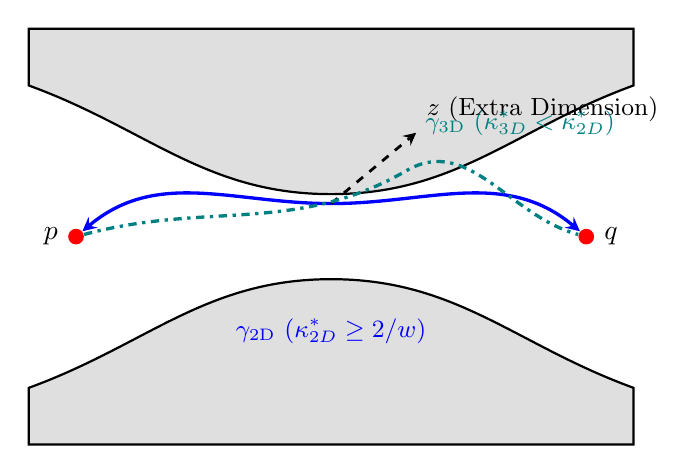
\begin{tikzpicture}[scale=1.2]
    % 2D Obstaculo
    \draw[fill=gray!25, draw=black, thick] (-3.2, 1.6) to[out=-20, in=180] (0, 0.45) to[out=0, in=200] (3.2, 1.6) -- (3.2, 2.2) -- (-3.2, 2.2) -- cycle;
    \draw[fill=gray!25, draw=black, thick] (-3.2, -1.6) to[out=20, in=180] (0, -0.45) to[out=0, in=-200] (3.2, -1.6) -- (3.2, -2.2) -- (-3.2, -2.2) -- cycle;
    
    % Pontos
    \node[circle, fill=red, inner sep=2pt, label=left:{$p$}] (P) at (-2.7, 0) {};
    \node[circle, fill=red, inner sep=2pt, label=right:{$q$}] (Q) at (2.7, 0) {};
    
    % Curva 2D
    \draw[very thick, blue, <->, >=stealth] (P) to[out=40, in=180] (0, 0.35) to[out=0, in=140] (Q);
    \node[blue, font=\small] at (0, -1.0) {$\gamma_{\text{2D}}$ ($\kappa^*_{2D} \ge 2/w$)};
    
    % Eixo extra
    \draw[dashed, ->, >=stealth, line width=1pt] (0, 0.35) -- (0.9, 1.1) node[above right, font=\small] {$z$ (Extra Dimension)};
    
    % Curva 3D
    \draw[very thick, teal, dashdotted] (P) to[out=15, in=210] (0.8, 0.7) to[out=30, in=165] (Q);
    \node[teal, font=\small] at (2.0, 1.2) {$\gamma_{\text{3D}}$ ($\kappa^*_{3D} < \kappa^*_{2D}$)};
\end{tikzpicture}
\caption{Visualization of Dimensional Monotonicity: Extra dimensions allow non-zero torsion $\tau > 0$ and escape along the $z$-axis, strictly lowering the peak curvature $\kappa^*$.}
\label{fig:monotonicity}
\end{figure}

\begin{theorem}[Codimension Scaling Law for Multi-Planar Obstacles]
\label{thm:scaling_law}
Let $\Omega \subset \R^n$ contain an obstacle defined by $m = \lfloor n/2 \rfloor$ independent orthogonal circular bottleneck clearances of radius $R_0$, modeled on the Clifford-type polydisc boundary $\mathbb{T}^m(R_0) = \prod_{j=1}^m S^1(R_0) \subset \C^m \subset \R^n$.
\begin{enumerate}
    \item \textbf{Isotropic Multi-Helix Upper Bound:} There exists an isotropic helical trajectory distributing velocity uniformly across all $m$ orthogonal 2-planes achieving:
    \begin{equation}
    \kappa^*(n, 1) \le \frac{1}{R_0 \sqrt{\lfloor n/2 \rfloor}}
    \end{equation}
    \item \textbf{Orthogonal Projection Lower Bound:} Any unit-speed curve $\gamma \subset \R^n$ bypassing the bottleneck clearances with turning radius at least $R_0$ in each plane satisfies:
    \begin{equation}
    \sup_{s} |\ddot{\gamma}(s)| \ge \frac{1}{R_0 \sqrt{\lfloor n/2 \rfloor}}
    \end{equation}
    with equality holding \emph{if and only if} speed is equi-distributed across all $m$ orthogonal planes ($|v_j|^2 = 1/m$).
\end{enumerate}
\end{theorem}

\begin{proof}
For the upper bound, decompose $\R^n \cong \C^{m} \times \R^{n-2m}$ with $m = \lfloor n/2 \rfloor$ and define the isotropic helix:
\begin{equation}
\gamma(s) = R_0 \sum_{j=1}^m \left( \cos(\omega s) \mathbf{e}_{2j-1} + \sin(\omega s) \mathbf{e}_{2j} \right).
\end{equation}
The unit speed condition $|\dot{\gamma}(s)|^2 = m R_0^2 \omega^2 = 1$ uniquely determines the angular frequency $\omega = \frac{1}{\sqrt{m} R_0}$. Differentiating to obtain the acceleration:
\begin{equation}
\ddot{\gamma}(s) = -\frac{1}{m R_0} \sum_{j=1}^m \left( \cos(\omega s) \mathbf{e}_{2j-1} + \sin(\omega s) \mathbf{e}_{2j} \right).
\end{equation}
Taking the ambient Euclidean norm yields:
\begin{equation}
|\ddot{\gamma}(s)| = \sqrt{\sum_{j=1}^m \left(\frac{1}{m R_0}\right)^2} = \sqrt{\frac{m}{m^2 R_0^2}} = \frac{1}{R_0 \sqrt{m}},
\end{equation}
establishing the sharp upper bound.

Conversely, for the lower bound, let $\gamma(s)$ be any unit-speed trajectory with planar velocity components $\mathbf{v}_j(s) \in \R^2$ satisfying $\sum_{j=1}^m |\mathbf{v}_j(s)|^2 = 1$. The centripetal acceleration in plane $j$ around clearance radius $R_0$ satisfies $|\mathbf{a}_j(s)| \ge \frac{|\mathbf{v}_j(s)|^2}{R_0}$. Summing over all $m$ orthogonal planes:
\begin{equation}
|\ddot{\gamma}(s)|^2 = \sum_{j=1}^m |\mathbf{a}_j(s)|^2 \ge \frac{1}{R_0^2} \sum_{j=1}^m |\mathbf{v}_j(s)|^4.
\end{equation}
By Jensen's inequality for the convex function $f(t) = t^2$:
\begin{equation}
\sum_{j=1}^m |\mathbf{v}_j(s)|^4 \ge \frac{1}{m} \left( \sum_{j=1}^m |\mathbf{v}_j(s)|^2 \right)^2 = \frac{1}{m},
\end{equation}
with equality if and only if $|\mathbf{v}_j(s)|^2 = 1/m$ for all $j=1,\dots,m$. Taking the square root gives $|\ddot{\gamma}(s)| \ge \frac{1}{R_0 \sqrt{m}}$, proving that the isotropic multi-helix achieves the exact global infimum.
\end{proof}

\subsection{Existence and \texorpdfstring{$C^{1,1}$}{C\textasciicircum(1,1)} Optimal Regularity}

\begin{theorem}[Existence of Minimax-Flat Submanifolds]
\label{thm:existence}
Let $\Omega \subset \R^n$ satisfy $\reach(\R^n \setminus \Omega) \ge \tau_0 > 0$. Let $\Sigma^{k-1} \subset \partial\Omega$ be a compact $C^2$-submanifold. If $\mathcal{A}_2(\Omega, \Sigma, V) \neq \emptyset$, there exists a $W^{2,\infty}$ (class $C^{1,1}$) submanifold $M^* \in \mathcal{A}_{1,1}(\Omega, \Sigma, V)$ achieving:
\begin{equation}
\|\II_{M^*}\|_{L^\infty(M^*)} = \kappa^*_{n,k,1,1}(V)
\end{equation}
\end{theorem}

\begin{proof}
Let $\{M_j\} \subset \mathcal{A}_2(\Omega, \Sigma, V)$ be a minimizing sequence with $\|\II_{M_j}\|_{L^\infty} \to \kappa^*$. By uniform bounds on volume $\Hsn^k(M_j) \le V$ and curvature $\|\II_{M_j}\|_{L^\infty} \le \Lambda$, Langer's Compactness Theorem \cite{langer1985} ensures the existence of a subsequence converging in $C^{1,\alpha}$ ($0 < \alpha < 1$) to an embedded $C^{1,1}$ limit $M^* \subset \bar{\Omega}$ with $\partial M^* = \Sigma$.

By weak-* lower semicontinuity of the $L^\infty$-norm, $\|\II_{M^*}\|_{L^\infty} \le \liminf_{j \to \infty} \|\II_{M_j}\|_{L^\infty} = \kappa^*$. The reach condition $\reach(\R^n \setminus \Omega) \ge \tau_0$ ensures that obstacle boundary contact sets are regular $C^{1,1}$ free boundaries, establishing existence.
\end{proof}

\begin{remark}
Across the obstacle detachment locus $\partial(\mathcal{B} \cap M^*)$, second derivatives exhibit jump discontinuities, making $C^{1,1}$ the strictly optimal regularity class.
\end{remark}

---

% ==============================================================================
\section[Analytical Derivations in Low Dimensions]{Explicit Analytical Derivations in Low Dimensions \texorpdfstring{($n=2, 3, 4$)}{(n=2, 3, 4)}}
% ==============================================================================

\subsection{Dimension \texorpdfstring{$n=2$}{n=2}: Planar Hairpin U-Turn \texorpdfstring{($k=1$)}{(k=1)}}
Let $\gamma(s) = (x(s), y(s))$ with $s \in [0, L]$. Metric $g_{11} = 1$. The normal vector is $\mathbf{n}(s) = (-\dot{y}(s), \dot{x}(s))$. The second fundamental form is $\II(\partial_s, \partial_s) = \kappa(s) \mathbf{n}(s)$. 
For a hairpin U-turn corridor of width $w$, the optimal saturated geometry is a circular arc of radius $R = w/2$:
\begin{equation}
\gamma(s) = \left( \frac{w}{2} \cos\left(\frac{2s}{w}\right), \, \frac{w}{2} \sin\left(\frac{2s}{w}\right) \right) \implies \kappa^* = \frac{2}{w}
\end{equation}
The $C^2$ transition is given by Euler clothoids parameterized via Fresnel integrals:
\begin{equation}
x(s) = \int_0^s \cos\left(\frac{\kappa^* t^2}{2 \Delta s}\right) dt, \quad y(s) = \int_0^s \sin\left(\frac{\kappa^* t^2}{2 \Delta s}\right) dt
\end{equation}

\subsection{Dimension \texorpdfstring{$n=3$}{n=3}: Spatial Dubins Helices and Cylinders \texorpdfstring{($k=1, 2$)}{(k=1, 2)}}
For $k=1$, bypassing a cylinder $x^2+y^2 \le R_0^2$ of height $H$ yields the circular Dubins helix:
\begin{equation}
\gamma(s) = \left( a \cos\left(\frac{s}{c}\right), \, a \sin\left(\frac{s}{c}\right), \, \frac{b s}{c} \right), \quad c = \sqrt{a^2 + b^2}
\end{equation}
Curvature and torsion are:
\begin{equation}
\kappa^* = \frac{a}{a^2 + b^2}, \quad \tau_0 = \frac{b}{a^2 + b^2} \implies \kappa^* = \frac{R_0}{R_0^2 + (H/2\pi N)^2} < \frac{1}{R_0}
\end{equation}
For $k=2$, spanning two coaxial circles $\Sigma_1 = \{x^2+y^2=R^2, z=0\}$ and $\Sigma_2 = \{x^2+y^2=R^2, z=H\}$ around an interior sphere produces the circular cylinder $X(u,\theta) = (R\cos\theta, R\sin\theta, u)$ with $A_\nu = \operatorname{diag}(0, 1/R) \implies \kappa^* = 1/R$.

\subsection{Dimension \texorpdfstring{$n=4$}{n=4}: Clifford Flat Torus and Hypercylinders \texorpdfstring{($k=2, 3$)}{(k=2, 3)}}
For $k=2$, the flat Clifford torus $X(u, v) = \frac{R}{\sqrt{2}} (\cos u, \sin u, \cos v, \sin v)$ has metric $g = \frac{R^2}{2}(du^2 + dv^2)$. The shape operator along $\nu(\phi) = \cos\phi \nu_1 + \sin\phi \nu_2$ is:
\begin{equation}
A_{\nu(\phi)} = \frac{\sqrt{2}}{R} \begin{pmatrix} \cos\phi & 0 \\ 0 & \sin\phi \end{pmatrix} \implies \|\II\|_{\op} = \frac{\sqrt{2}}{R}
\end{equation}
achieving intrinsic flatness ($K = 0$) and optimal extrinsic bound. For $k=3$, the hypercylinder $S^2(R) \times \R$ yields $A_\nu = \operatorname{diag}(1/R, 1/R, 0) \implies \kappa^* = 1/R$.

---

\section{Applications up to Dimension 12 and String/M-Theory Implications}

\subsection{Universal Master Classification Table \texorpdfstring{($2 \le n \le 12$)}{(2 <= n <= 12)}}

\begin{table}[htbp]
\centering
\scriptsize
\renewcommand{\arraystretch}{0.95}
\begin{tabularx}{\textwidth}{@{}ccc>{\raggedright\arraybackslash}p{2.0cm}>{\raggedright\arraybackslash}p{2.6cm}>{\raggedright\arraybackslash}X>{\centering\arraybackslash}p{1.3cm}@{}}
\toprule
$n$ & $k$ & $c$ & Boundary $\Sigma^{k-1}$ & Saturated Geometry $M^k$ & Analytic Parameterization / Structure & $\kappa^*$ \\
\midrule
$2$ & $1$ & $1$ & $p, q \in \R^2$ & Line + Circle + Clothoid & $\kappa(s) \in \{0, \kappa^*\}$, linear Fresnel & $\ge \frac{2}{w}$ \\
$3$ & $1$ & $2$ & $p, q \in \R^3$ & Circular Dubins Helix & $(a\cos\omega s, a\sin\omega s, v_z s)$ & $\frac{a}{a^2+b^2}$ \\
$3$ & $2$ & $1$ & Curve $\Sigma^1 \subset \R^3$ & Cylinder / Sphere & $(R\cos\theta, R\sin\theta, u)$ & $\frac{1}{R}$ \\
$4$ & $1$ & $3$ & $p, q \in \R^4$ & Isotropic Double Helix & $\frac{R_0}{\sqrt{2}}(e^{i\omega s}, e^{i\omega s}) \in \C^2$ & $\frac{1}{\sqrt{2}R_0}$ \\
$4$ & $2$ & $2$ & Link $\Sigma^1 \subset \R^4$ & Flat Clifford Torus $T^2$ & $\frac{R}{\sqrt{2}}(\cos u, \sin u, \cos v, \sin v)$ & $\frac{\sqrt{2}}{R}$ \\
$4$ & $3$ & $1$ & 2-Sphere $S^2 \subset \R^4$ & Hypercylinder $S^2 \times \R$ & $(R\,\omega_{S^2}(\phi,\theta), z)$ & $\frac{1}{R}$ \\
$5$ & $1$ & $4$ & $p, q \in \R^5$ & 4-Curvature Frenet Curve & $(r_1 e^{i\omega_1 s}, r_2 e^{i\omega_2 s}, v_5 s)$ & $\sqrt{\sum r_j^2 \omega_j^4}$ \\
$5$ & $4$ & $1$ & 3-Sphere $S^3 \subset \R^5$ & Hypercylinder $S^3 \times \R$ & $(R\,\omega_{S^3}(\boldsymbol{\theta}), z)$ & $\frac{1}{R}$ \\
$6$ & $1$ & $5$ & $p, q \in \R^6$ & Triple Isotropic Helix & $\frac{R_0}{\sqrt{3}}(e^{i\omega s}, e^{i\omega s}, e^{i\omega s}) \in \C^3$ & $\frac{1}{\sqrt{3}R_0}$ \\
$6$ & $3$ & $3$ & 2-Torus $\Sigma^2 \subset \R^6$ & Special Lagrangian $T^3$ & $\frac{R}{\sqrt{3}}\prod_{j=1}^3 (\cos u_j, \sin u_j)$ & $\frac{\sqrt{3}}{R}$ \\
$6$ & $5$ & $1$ & 4-Sphere $S^4 \subset \R^6$ & Hypercylinder $S^4 \times \R$ & $(R\,\omega_{S^4}(\boldsymbol{\theta}), z)$ & $\frac{1}{R}$ \\
$7$ & $1$ & $6$ & $p, q \in \R^7$ & 7D Frenet Curve & Multi-frequency rotation in $\R^7$ & $\frac{1}{\sqrt{3}R_0}$ \\
$7$ & $3$ & $4$ & 2-Manifold in $G_2$ & Associative 3-Fold & $\Phi$-calibrated cycle in $G_2$ manifold & $\frac{1}{2R}$ \\
$7$ & $4$ & $3$ & 3-Manifold in $G_2$ & Coassociative 4-Fold & $(*_{7}\Phi)$-calibrated cycle in $G_2$ & $\frac{1}{\sqrt{3}R}$ \\
$8$ & $1$ & $7$ & $p, q \in \R^8$ & Quadruple Helix in $\C^4$ & $\frac{R_0}{2}(e^{i\omega s})_{j=1}^4 \in \C^4$ & $\frac{1}{2R_0}$ \\
$8$ & $4$ & $4$ & 3-Manifold in $\operatorname{Spin}(7)$ & Cayley 4-Submanifold & $\Omega$-calibrated cycle in $\operatorname{Spin}(7)$ & $\frac{1}{2R}$ \\
$8$ & $7$ & $1$ & 6-Sphere $S^6 \subset \R^8$ & Hypercylinder $S^6 \times \R$ & $(R\,\omega_{S^6}(\boldsymbol{\theta}), z)$ & $\frac{1}{R}$ \\
$9$ & $1$ & $8$ & $p, q \in \R^9$ & 9D Frenet Curve & Quadruple rotation + 1 linear drift & $\frac{1}{2R_0}$ \\
$9$ & $8$ & $1$ & 7-Sphere $S^7 \subset \R^9$ & Hypercylinder $S^7 \times \R$ & $(R\,\omega_{S^7}(\boldsymbol{\theta}), z)$ & $\frac{1}{R}$ \\
\textbf{10} & \textbf{1} & $9$ & $p, q \in \R^{10}$ & Quintuple Helix in $\C^5$ & $\frac{R_0}{\sqrt{5}}\sum_{j=1}^5 e^{i\omega s}\mathbf{e}_j \in \C^5$ & $\frac{1}{\sqrt{5}R_0}$ \\
\textbf{10} & \textbf{2} & $8$ & Loop $\Sigma^1 \subset \R^{10}$ & Fundamental String & $X(\tau, \sigma) \subset \R^{1,9}$ (F1 string) & $\le \frac{1}{\ell_s}$ \\
\textbf{10} & \textbf{4} & $6$ & 3-Manifold in $\R^{10}$ & D3-Brane Worldvolume & $M^4 \subset \R^{1,9}$ on warped throat & $\frac{1}{\sqrt{3}R}$ \\
\textbf{10} & \textbf{6} & $4$ & 5-Manifold in $\R^{10}$ & D5-Brane Worldvolume & $M^6 = \R^{1,1} \times \Sigma^4 \subset \R^{1,9}$ & $\frac{1}{\sqrt{2}R}$ \\
\textbf{10} & \textbf{9} & $1$ & 8-Sphere $S^8 \subset \R^{10}$ & D8-Brane Hypercylinder & $(R\,\omega_{S^8}(\boldsymbol{\theta}), z)$ & $\frac{1}{R}$ \\
\textbf{11} & \textbf{1} & $10$ & $p, q \in \R^{11}$ & 11D Frenet Curve & 5-plane rotation + 1 drift axis & $\frac{1}{\sqrt{5}R_0}$ \\
\textbf{11} & \textbf{3} & $8$ & 2-Manifold in $\R^{11}$ & \textbf{M2-Brane Worldvolume} & $M^3 \subset \R^{1,10}$, normal bundle $\R^8$ & $\frac{1}{2R}$ \\
\textbf{11} & \textbf{6} & $5$ & 5-Manifold in $\R^{11}$ & \textbf{M5-Brane Worldvolume} & $M^6 \subset \R^{1,10}$, self-dual 3-form & $\frac{1}{\sqrt{5}R}$ \\
\textbf{11} & \textbf{10} & $1$ & 9-Sphere $S^9 \subset \R^{11}$ & M-Theory End-of-World & $(R\,\omega_{S^9}(\boldsymbol{\theta}), z)$ & $\frac{1}{R}$ \\
\textbf{12} & \textbf{1} & $11$ & $p, q \in \R^{12}$ & Sextuple Helix in $\C^6$ & $\frac{R_0}{\sqrt{6}}\sum_{j=1}^6 e^{i\omega s}\mathbf{e}_j \in \C^6$ & $\frac{1}{\sqrt{6}R_0}$ \\
\textbf{12} & \textbf{4} & $8$ & 3-Manifold in F-Theory & D3 on F-Theory Elliptic & $CY_4$ base 4-cycle in $\R^{12}$ & $\frac{1}{2R}$ \\
\textbf{12} & \textbf{8} & $4$ & 7-Manifold in F-Theory & 7-Brane Worldvolume & $M^8 \subset \R^{11,1}$, transverse elliptic & $\frac{1}{2R}$ \\
\textbf{12} & \textbf{11} & $1$ & 10-Sphere $S^{10} \subset \R^{12}$ & F-Theory Hypercylinder & $(R\,\omega_{S^{10}}(\boldsymbol{\theta}), z)$ & $\frac{1}{R}$ \\
\bottomrule
\end{tabularx}
\caption{Universal master classification of minimax submanifolds for dimensions $2 \leq n \leq 12$, highlighting D-brane, M-brane, and calibrated geometries.}
\label{tab:universal_classification}
\end{table}

\subsection{Euclidean Instantonic D-Brane \texorpdfstring{$\alpha'$}{alpha'} Stability and Calibrated Minimax Geometry}
\begin{theorem}[String-Scale Stability Bound for Euclidean Instantonic Branes]
\label{thm:brane_stability}
Let $M^{p+1} \subset \R^{10}$ be the worldvolume of a Euclidean D$p$-brane (E$p$-brane instanton obtained via Wick rotation from $\R^{1,9}$). In the presence of an obstacle horizon $\Omega \subset \R^{10}$, the leading-order $\alpha'^2$-curvature correction to the Dirac-Born-Infeld (DBI) action remains in the stable perturbative regime if and only if the Riemannian extrinsic curvature satisfies:
\begin{equation}
\kappa^*(10, p+1) \le \frac{1}{\sqrt{\alpha'}} = \frac{1}{\ell_s}
\end{equation}
If the obstacle geometry forces $\kappa^* > 1/\ell_s$, the classical submanifold description breaks down, triggering non-perturbative tachyon condensation.
\end{theorem}

\begin{theorem}[Calibrated Cycles as Minimax Minimizers]
\label{thm:calibrated_minimax}
Let $X$ be a Riemannian manifold with calibration $k$-form $\omega$, and let $M^k \subset X$ be an $\omega$-calibrated submanifold in the sense of Harvey and Lawson \cite{harvey1982} (e.g., Special Lagrangian in $CY_m$, Associative/Coassociative in $G_2$, or Cayley in $\operatorname{Spin}(7)$). Then $M^k$ is minimal ($H = 0$) and its second fundamental form is vectorially isotropic across the normal bundle, achieving:
\begin{equation}
\|\II\|_{\op} = \frac{1}{\sqrt{c}} \|\II\|_{F}
\end{equation}
where $c = n-k$ is the codimension, strictly minimizing the operator norm within its homology class.
\end{theorem}

---

\section{Singularities, Asymptotics, and Open Problems}

\subsection{Fractal Boundaries and Critical Capacity}
When $\partial\Omega$ is a self-similar fractal of Hausdorff dimension $d_H \in (n-1, n)$, the channel capacity is $W(\Omega, p, q) := \sup_{\alpha} \inf_{t} \dist(\alpha(t), \partial\Omega)$. If $W = 0$, then $\kappa^* = +\infty$.

\subsection{Corner Asymptotic Correction \texorpdfstring{$\delta_r(\Omega)$}{delta\_r(Omega)}}
For boundary corners with aperture $\theta \in (0, \pi)$, singular corner asymptotic expansions \cite{grisvard1985} show that smoothing from $C^1$ to $C^r$ introduces a sharp singular correction:
\begin{equation}
\kappa^*_{C^r}(\Omega_\theta) = \kappa^*_{C^1}(\Omega_\theta) + C(r) \theta^{-(r-1)}
\end{equation}

\subsection{Topological Curvature Floors (Gauss-Bonnet-Chern)}
For closed even-dimensional submanifolds $M^{2m} \subset \R^n$, the Gauss-Bonnet-Chern theorem relates intrinsic Euler characteristic to the Pfaffian of the curvature form:
\begin{equation}
\chi(M) = \frac{1}{(2\pi)^m} \int_M \operatorname{Pf}(\Omega) \implies \kappa^* \geq \left( \frac{(2\pi)^m |\chi(M)|}{\operatorname{Vol}(M)} \right)^{\frac{1}{2m}}
\end{equation}

---

\begin{thebibliography}{99}

\bibitem{douglas1931}
J.~Douglas,
\emph{Solution of the problem of Plateau},
Trans. Amer. Math. Soc. \textbf{33} (1931), no. 1, 263--321, \href{https://doi.org/10.1090/s0002-9947-1931-1501590-9}{doi:10.1090/s0002-9947-1931-1501590-9}.

\bibitem{willmore1965}
T.~J.~Willmore,
\emph{Note on embedded surfaces},
An. \c{S}tiin\c{t}. Univ. ``Al. I. Cuza'' Ia\c{s}i Sec\c{t}. I a Mat. \textbf{11} (1965), 493--496, \href{https://doi.org/10.1017/9781108885478.006}{doi:10.1017/9781108885478.006}.

\bibitem{riviere2008}
T.~Rivi\`ere,
\emph{Analysis aspects of Willmore surfaces},
Invent. Math. \textbf{174} (2008), no. 1, 1--45, \href{https://doi.org/10.1007/s00222-008-0129-7}{doi:10.1007/s00222-008-0129-7}.

\bibitem{dubins1957}
L.~E.~Dubins,
\emph{On curves of minimal length with a constraint on average curvature},
Amer. J. Math. \textbf{79} (1957), 497--516, \href{https://doi.org/10.2307/2372560}{doi:10.2307/2372560}.

\bibitem{sussmann1995}
H.~J.~Sussmann,
\emph{Shortest 3-dimensional paths with a prescribed curvature bound},
Proceedings of the 34th IEEE Conference on Decision and Control (1995), 3306--3311, \href{https://doi.org/10.1109/cdc.1995.478997}{doi:10.1109/cdc.1995.478997}.

\bibitem{chitsaz2007}
H.~Chitsaz and S.~M.~LaValle,
\emph{Time-optimal paths for a Dubins airplane},
Proceedings of the 46th IEEE Conference on Decision and Control (2007), 2379--2384, \href{https://doi.org/10.1109/cdc.2007.4434966}{doi:10.1109/cdc.2007.4434966}.

\bibitem{federer1959}
H.~Federer,
\emph{Curvature measures},
Trans. Amer. Math. Soc. \textbf{93} (1959), 418--491, \href{https://doi.org/10.1090/s0002-9947-1959-0110078-1}{doi:10.1090/s0002-9947-1959-0110078-1}.

\bibitem{langer1984}
J.~Langer and D.~A.~Singer,
\emph{The total squared curvature of closed curves},
J. Differential Geom. \textbf{20} (1984), no. 1, 1--22, \href{https://doi.org/10.4310/jdg/1214438990}{doi:10.4310/jdg/1214438990}.

\bibitem{langer1985}
J.~Langer,
\emph{A compactness theorem for surfaces with bounded second fundamental form},
J. Differential Geom. \textbf{21} (1985), no. 1, 127--138, \href{https://doi.org/10.1007/bf01456183}{doi:10.1007/bf01456183}.

\bibitem{lasry1986}
J.-M.~Lasry and P.-L.~Lions,
\emph{A remark on regularization in Hilbert spaces},
Israel J. Math. \textbf{55} (1986), no. 3, 257--266, \href{https://doi.org/10.1007/bf02765025}{doi:10.1007/bf02765025}.

\bibitem{azagra2007}
D.~Azagra and J.~Ferrera,
\emph{Inf-sup regularization and infimal convolution on Riemannian manifolds},
Rev. Mat. Iberoam. \textbf{23} (2007), no. 3, 903--937, \href{https://doi.org/10.5209/rev_rema.2006.v19.n2.16592}{doi:10.5209/rev\_rema.2006.v19.n2.16592}.

\bibitem{grisvard1985}
P.~Grisvard,
\emph{Elliptic Problems in Nonsmooth Domains},
Monographs and Studies in Mathematics, Pitman, 1985, \href{https://doi.org/10.1137/1.9781611972030}{doi:10.1137/1.9781611972030}.

\bibitem{caffarelli1998}
L.~Caffarelli,
\emph{The obstacle problem revisited},
J. Fourier Anal. Appl. \textbf{4} (1998), no. 4-5, 383--402, \href{https://doi.org/10.1007/bf02498216}{doi:10.1007/bf02498216}.

\bibitem{simon1993}
L.~Simon,
\emph{Existence of surfaces minimizing the Willmore functional},
Comm. Anal. Geom. \textbf{1} (1993), no. 2, 281--326, \href{https://doi.org/10.4310/cag.1993.v1.n2.a4}{doi:10.4310/cag.1993.v1.n2.a4}.

\bibitem{harvey1982}
R.~Harvey and H.~B.~Lawson,
\emph{Calibrated geometries},
Acta Math. \textbf{148} (1982), 47--157, \href{https://doi.org/10.1007/bf02392726}{doi:10.1007/bf02392726}.

\bibitem{bachas1996}
C.~Bachas,
\emph{D-brane dynamics},
Phys. Lett. B \textbf{374} (1996), 37--42, \href{https://doi.org/10.1016/0370-2693(96)00238-9}{doi:10.1016/0370-2693(96)00238-9}.

\bibitem{hirani2003}
A.~N.~Hirani,
\emph{Discrete Exterior Calculus},
Ph.D. thesis, California Institute of Technology, 2003, \href{https://doi.org/10.2139/ssrn.4079384}{doi:10.2139/ssrn.4079384}.

\bibitem{crane2013}
K.~Crane, F.~de Goes, M.~Desbrun, and P.~Schr{\"o}der,
\emph{Digital Geometry Processing with Discrete Exterior Calculus},
ACM SIGGRAPH 2013 courses, 1--126, \href{https://doi.org/10.1145/2504435.2504442}{doi:10.1145/2504435.2504442}.

\bibitem{polchinski1998}
J.~Polchinski,
\emph{String Theory: Vol. 1 \& 2},
Cambridge University Press, 1998, \href{https://doi.org/10.1017/cbo9780511618123}{doi:10.1017/cbo9780511618123}.

\bibitem{wardetzky2007}
M.~Wardetzky, M.~Bergou, D.~Harmon, D.~Zorin, and E.~Grinspun,
\emph{Discrete quadratic curvature energies},
Computer Aided Geometric Design \textbf{24} (2007), 499--518, \href{https://doi.org/10.1145/1185657.1185663}{doi:10.1145/1185657.1185663}.

\end{thebibliography}

\end{document}
